\documentclass[
	12pt,				% tamanho da fonte
	oneside,			% para impressão em recto e verso. Oposto a oneside
	a4paper,			% tamanho do papel. 
	english,			% idioma adicional para hifenização
	brazil,				% o último idioma é o principal do documento
	]{abntex2}

% ---
% Pacotes fundamentais 
% ---
\usepackage{lmodern}			% Usa a fonte Latin Modern
\usepackage[T1]{fontenc}		% Selecao de codigos de fonte.
\usepackage[utf8]{inputenc}		% Codificacao do documento (conversão automática dos acentos)
\usepackage{indentfirst}		% Indenta o primeiro parágrafo de cada seção.
\usepackage{color}				% Controle das cores
\usepackage{graphicx}			% Inclusão de gráficos
\usepackage{microtype} 			% para melhorias de justificação
\usepackage{multicol}
\usepackage{multirow}
\usepackage[brazilian,hyperpageref]{backref}	 % Paginas com as citações na bibl
\usepackage[alf]{abntex2cite}	% Citações padrão ABNT
\usepackage{float}

% --- 
% CONFIGURAÇÕES DE PACOTES
% --- 

% ---
% Configurações do pacote backref
% Usado sem a opção hyperpageref de backref
\renewcommand{\backrefpagesname}{Citado na(s) página(s):~}
% Texto padrão antes do número das páginas
\renewcommand{\backref}{}
% Define os textos da citação
\renewcommand*{\backrefalt}[4]{
	\ifcase #1 %
		Nenhuma citação no texto.%
	\or
		Citado na página #2.%
	\else
		Citado #1 vezes nas páginas #2.%
	\fi}%
% ---

% ---
% Informações de dados para CAPA e FOLHA DE ROSTO
% ---
\titulo{Prática 15\\Laboratório de AEDS}
\autor{Pedro Inácio Rodrigues Pontes}
\local{Belo Horizonte, Brasil}
\data{2024}
\instituicao{%
  Universidade Federal de Minas Gerais
  \par
  Colégio Técnico
  \par
  Curso Técnico em Desenvolvimento de Sistemas}

\definecolor{blue}{RGB}{41,5,195}

\makeatletter
\hypersetup{
     	%pagebackref=true,
		pdftitle={\@title}, 
		pdfauthor={\@author},
    	pdfsubject={\imprimirpreambulo},
		colorlinks=true,       		% false: boxed links; true: colored links
    	linkcolor=blue,          	% color of internal links
    	citecolor=blue,        		% color of links to bibliography
    	filecolor=magenta,      		% color of file links
		urlcolor=blue,
		bookmarksdepth=4
}
\makeatother

\renewcommand{\thesection}{\arabic{section}}
\setlength{\parindent}{1.3cm}
\setlength{\parskip}{0.2cm} 

\makeindex


\begin{document}

\selectlanguage{brazil}
\frenchspacing 

\imprimircapa

{
\ABNTEXchapterfont

\textual

% ----------------------------------------------------------
% Introdução (exemplo de capítulo sem numeração, mas presente no Sumário)
% ----------------------------------------------------------
\section{Introdução}

    Foi disponibilizado um código que criava um grid infinito no ambiente de programação Processing, ao clicar com o botão esquerdo em uma célula do grid, ela fica preta. Clicando com o botão direito ela fica branca (vazia) novamente. O código permitia movimentação dentro do grid a partir do segurar e arrastar o mouse. E também permitia o zoom, ao mover a roda do mouse.

    O problema principal é a implementação de uma nova feature ao código, que é colocar um ciclo de cores para aparecer com os cliques do mouse, ao invés de apenas a cor preta.
    
    A implementação dos conhecimentos de dicionários adquiridos nas aulas de Algoritmo e Estrutura de Dados é necessária para resolver o problema, pois, como o grid é infinito, não seria possível nem prático usar um array de valores guardando o valor de cada célula, ao invés disso, é necessário o uso de um diciónario que armazena a posição e as cores de cada célula.

    Portanto, foi objetivada a implementação da mudança cíclica de cores ao clique no botão direito do mouse utilizando a estrutura dicionários, que já foi implementada inicialmente, o necessário era apenas construir código em volta dela utilizando suas características. Vale a pena lembrar que a cor branca não é guardada. O ciclo de cores é: preto, verde, vermelho, azul, amarelo e branco.

\section{Desenvolvimento}

Segue o código adicionado, com - significando que a linha foi removida e +, que foi adicionada, se não houver nada, ela já existia antes no código.

\begin{verbatim}
     if (mouseButton == LEFT) {
       // Botão esquerdo: preenche a célula com uma cor aleatória
       int novaCor = color(0);
-      coresCelulas.put(chave, novaCor);
+
+      if  (coresCelulas.containsKey(chave)) {
+
+        if (coresCelulas.get(chave) == color(0)) {
+          novaCor = color(0, 255, 0);
+        } else if (coresCelulas.get(chave) == color(0, 255, 0)) {
+          novaCor = color(255, 0, 0);
+        } else if (coresCelulas.get(chave) == color(255, 0, 0)) {
+          novaCor = color(0, 0, 255);
+        } else if (coresCelulas.get(chave) == color(0, 0, 255)) {
+          novaCor = color(255, 255, 0);
+        }
+        if (coresCelulas.get(chave) == color(255, 255, 0)) {
+          coresCelulas.remove(chave);
+        }
+      } else {
+        coresCelulas.put(chave, color(0));
+      }
+      if  (coresCelulas.containsKey(chave))
+        coresCelulas.put(chave, novaCor);
}
\end{verbatim}

Foi adicionado um if para observar se o diciónario coresCelulas contém a chave com que queremos trabalhar (a célula que clicamos). Se não a possuir, cairá no bloco else, onde colocaremos a chave com a cor preta (0) no diciónario. Se a chave já existir, isso indica que a célula em questão já foi clicada, portanto, será utilizado um bloco \textit{if else if} para averiguar qual a cor armzenada no hashmap (outra forma de se referir ao diciónario). O primeiro verificará se a cor é preta, se for, a variável local novaCor será atualizada para verde, essa verificação será repetida com todo o ciclo consecutivo de cores: se for verde a local será atualizada para vermelho, se vermelho para azul... A diferença mais marcante virá quando a cor for amarelo (255,255,0), nesse caso, a variável local não será atualizada, o hashmap da célula em questão que será removido. Isso levará à cor branca.

Após esse bloco if principal \textit{if  (coresCelulas.containsKey(chave))}, será feito outro if com os mesmos parâmetros, para atualizar o diciónario com a nova cor. Ele simplesmente chama o método put e coloca a nova cor para a chave. Esse código não pode ser acoplado ao primeiro if por haver o caso do amarelo para o branco, onde é removido o hashmap. Se esse acoplamento fosse feito, após ser removido, seria criado novamete o hashmap, fazendo a cor branca não ocorrer, já que ela só ocorre quando o diciónario para a célula não existe.

Observação: novaCor teve de ser inicializada com color(0) por haver um erro dizendo que ela não foi inicializada, tal ocorre no segundo if principal. Isso vêm do verificador de erros do Processing não conseguir averiguar se nova cor existirá com um valor válido quando o segundo if for chamado.

\section{Resultados}

\begin{figure}[H]
\centering

\includegraphics[width=0.4\textwidth]{imgs/img1.png}
\caption{Grid Inicial}
\label{Grid Inicial}
\end{figure}
\begin{figure}[H]
\centering
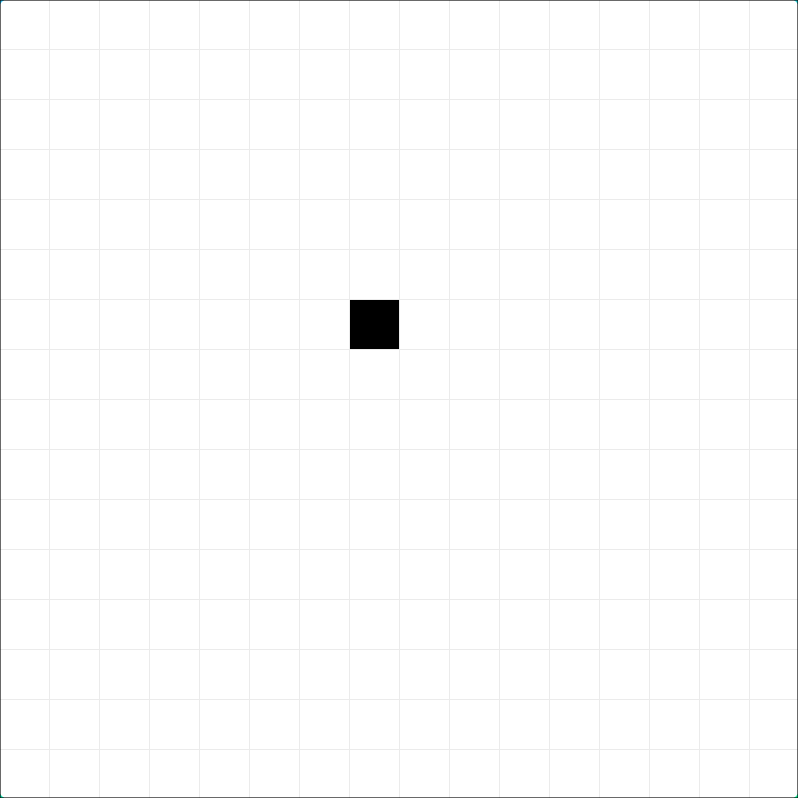
\includegraphics[width=0.4\textwidth]{imgs/img2.png}
\caption{Após clique nº1 na célula em questão}
\label{Após clique nº1 na célula em questão}
\end{figure}
\begin{figure}[H]
\centering
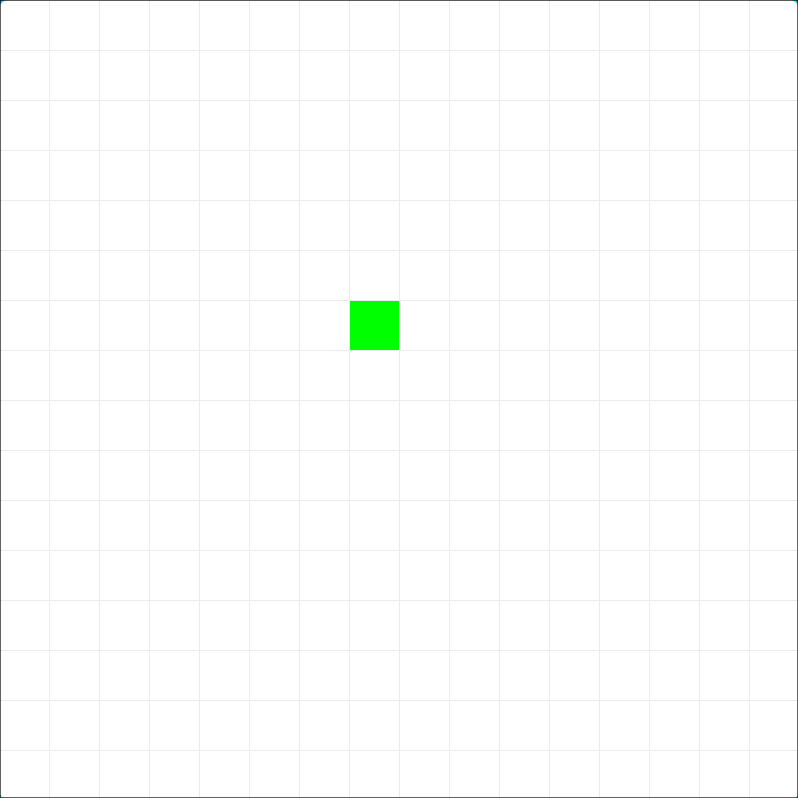
\includegraphics[width=0.4\textwidth]{imgs/img3.png}
\caption{Após clique nº2}
\label{Após clique nº2}
\end{figure}
\begin{figure}[H]
\centering
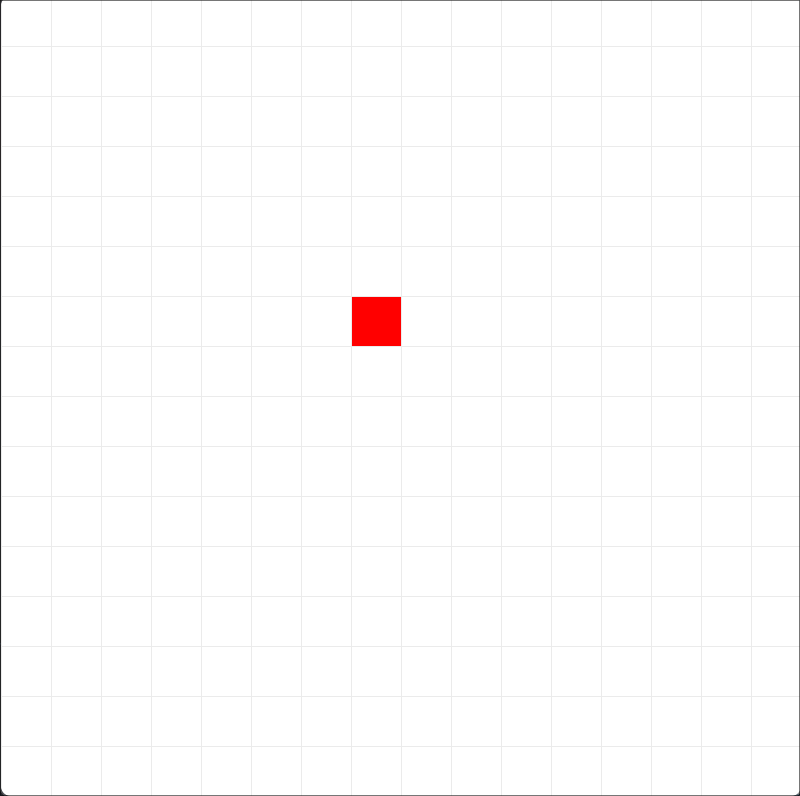
\includegraphics[width=0.4\textwidth]{imgs/img4.png}
\caption{Após clique nº3}
\label{Após clique nº3}
\end{figure}
\begin{figure}[H]
\centering
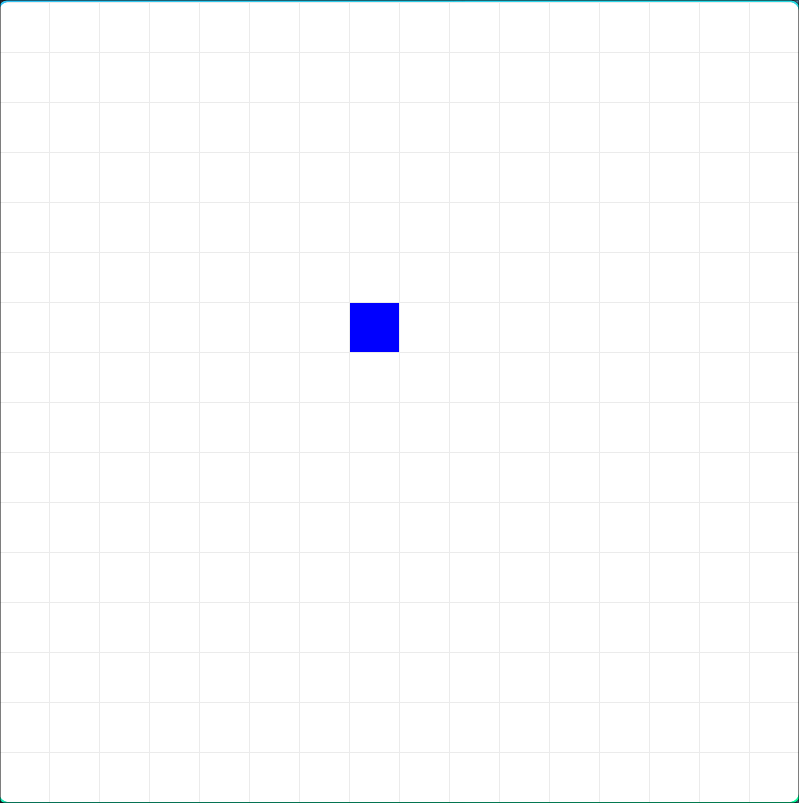
\includegraphics[width=0.4\textwidth]{imgs/img5.png}
\caption{Após clique nº4}
\label{Após clique nº4}
\end{figure}
\begin{figure}[H]
\centering
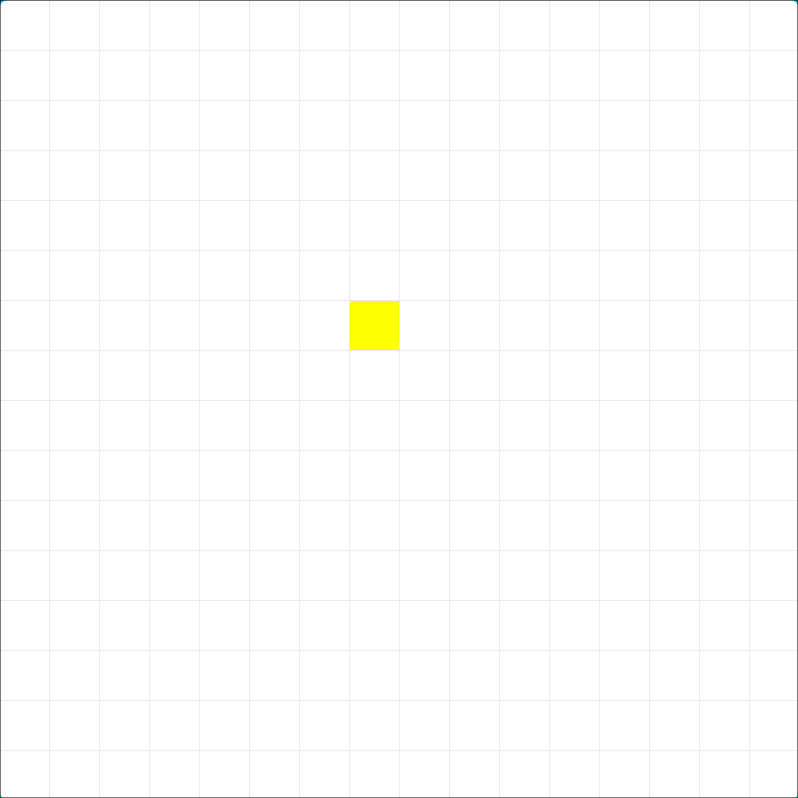
\includegraphics[width=0.4\textwidth]{imgs/img6.png}
\caption{Após clique nº5}
\label{Após clique nº5}
\end{figure}
\begin{figure}[H]
\centering

\includegraphics[width=0.4\textwidth]{imgs/img7.png}
\caption{Após clique nº6}
\label{Após clique nº6}
\end{figure}

\section{Conclusão}

\begin{itemize}
    \item Os objetivos foram devidamente alcançados.
    \item A maior dificuldade foi fazer a célula ficar branca, pois havia o conflito de ter que remover o diciónario nessa parte e após isso fazer ele não ser criado novamente até o próximo clique. Isso foi resolvido criando um if para ver se havia algo no dicionário e se houvesse, alterar a cor, onde o else levava à criação dele com a cor preta, e outro if que verificava a mesma coisa, mas se existisse ia ser colocada o variável local novaCor dentro do diciónario.
    \item Foi aprendido o uso prático dos hashmaps e dicionários, principalmente no que se trata aos métodos inerentes deles.
\end{itemize}


\end{document}
